\documentclass[12pt]{article}

\title{An visual method for generating the nonlinear separating isosurface of two classes of objects in two-dimensions using Marching Squares}
\author{
Shawn Halayka\footnote{Independent -- sjhalayka@gmail.com}
}


\date{\today\;\currenttime}

\usepackage{datetime}
\usepackage{listings}
\usepackage{cite}
\usepackage{xcolor}
\usepackage{graphicx}
\usepackage{setspace}
\usepackage{amsmath}
\usepackage{url}
\usepackage{amsfonts}
\usepackage{caption}
\usepackage{subcaption}

\usepackage[margin=1in]{geometry}

%\doublespace

\begin{document}




\maketitle

\begin{abstract}

\end{abstract}




\section{Introduction}

Iron out the wrinkles using blur.
Ameliorate


\pagebreak





\begin{thebibliography}{9}

\bibitem{mc} James, et al. An Introduction to Statistical Learning with Applications in R. ISBN: 978-1-0716-1417-4

\end{thebibliography}





\pagebreak






\begin{figure} 
\centering
  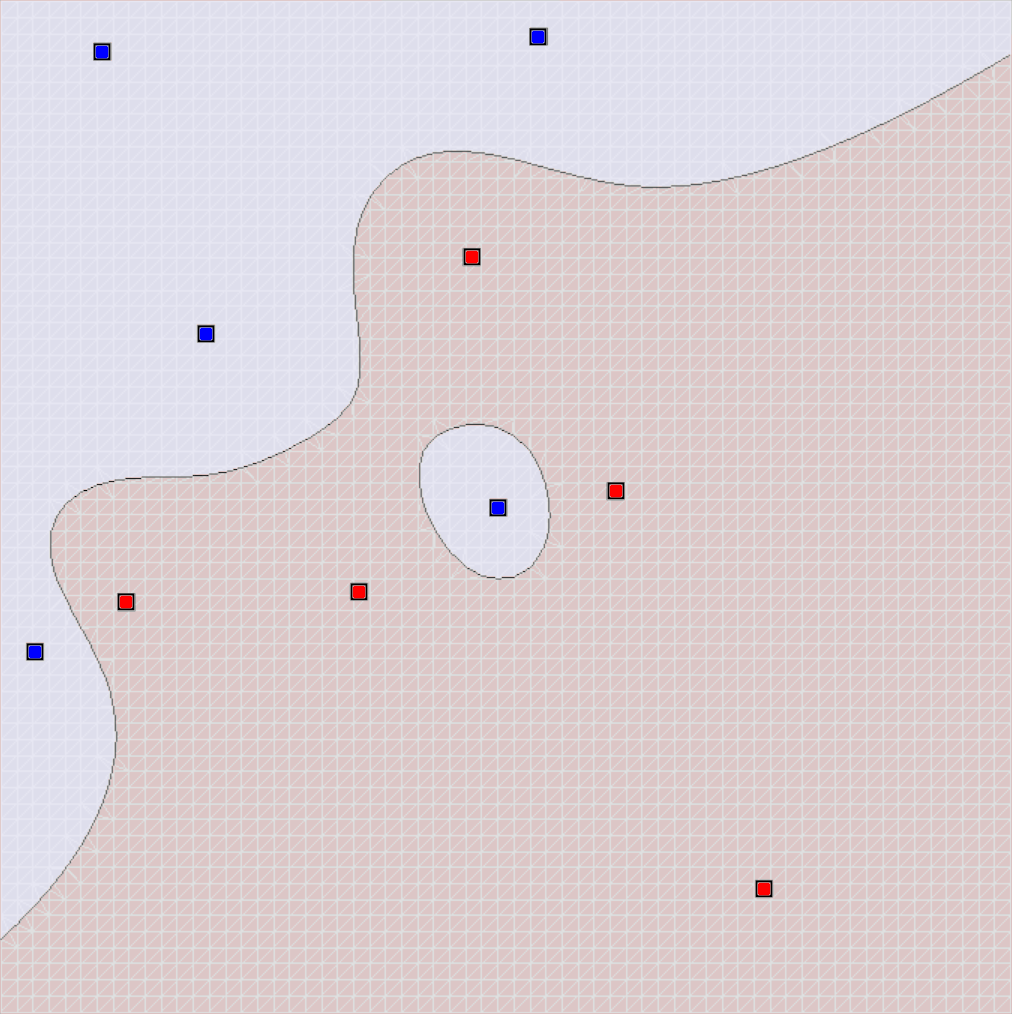
\includegraphics[width = 3 in]{64_res.png}
  \caption{Nonlinear separation.
}
\end{figure}

\begin{figure} 
\centering
  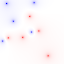
\includegraphics[width = 3 in]{64_res_image.png}
  \caption{Bitmap image used as input to the Marching Squares algorithm.
}
\end{figure}

\begin{figure} 
\centering
  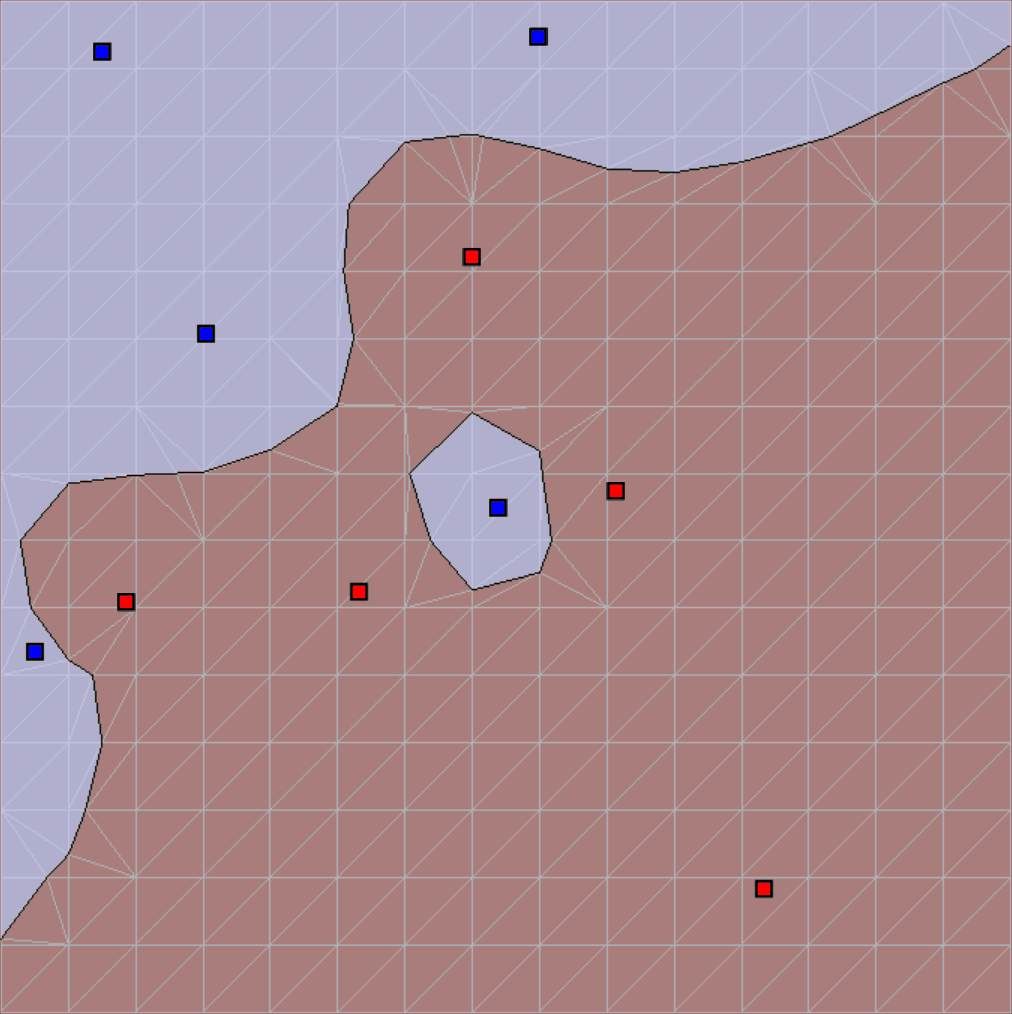
\includegraphics[width = 3 in]{16_res.png}
  \caption{Nonlinear separation.
}
\end{figure}

\begin{figure} 
\centering
  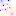
\includegraphics[width = 3 in]{16_res_image.png}
  \caption{Bitmap image used as input to the Marching Squares algorithm.
}
\end{figure}


\begin{figure} 
\centering
  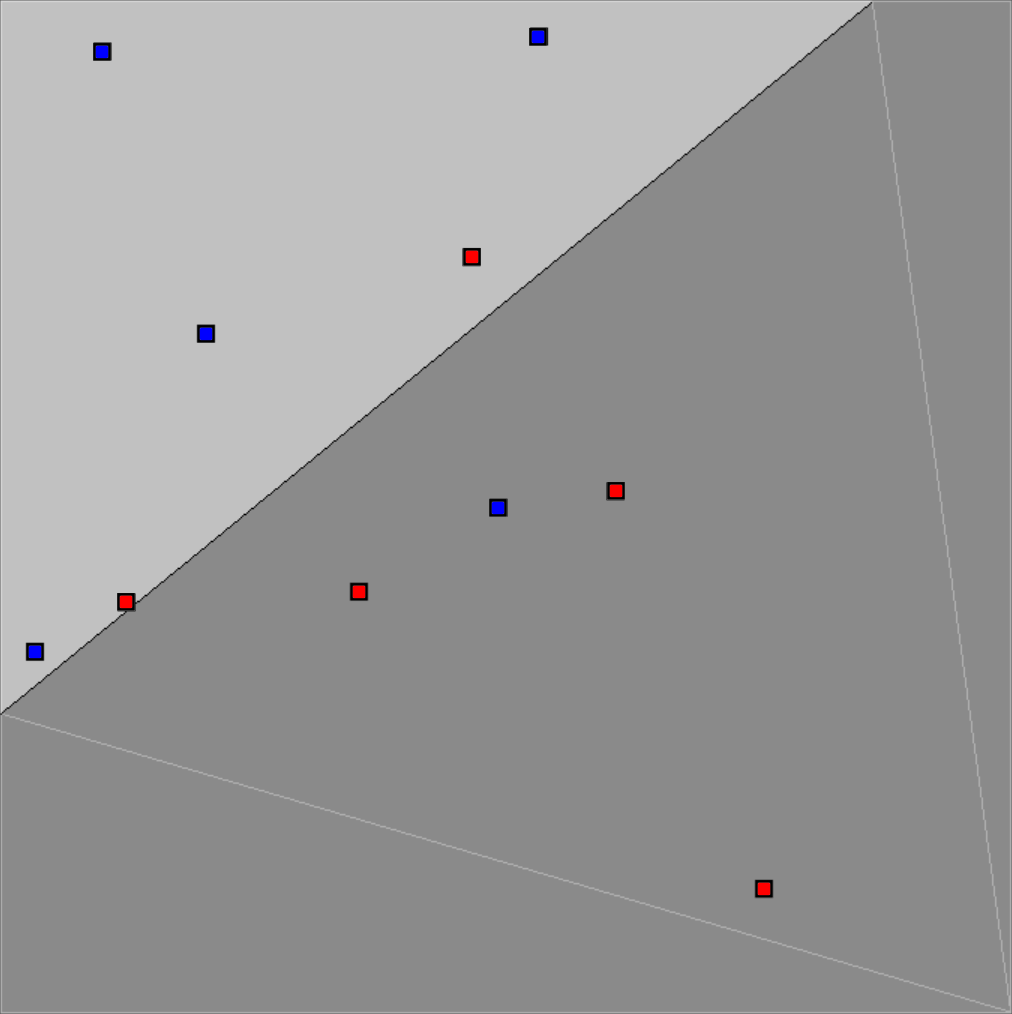
\includegraphics[width = 3 in]{2_res.png}
  \caption{Nonlinear separation.
}
\end{figure}

\begin{figure} 
\centering
  
\includegraphics[width = 3 in]{2_res_image.png}
  \caption{Bitmap image used as input to the Marching Squares algorithm.
}
\end{figure}


\end{document}









